\section{Introduction}
\label{cha:intro}

Classification is an important issue in machine learning and statistics. It has applications in many areas, as diverse as handwriting recognition, medicine, biometrics, computer vision, natural language processing, credit scoring etc. The task of classification is to identify the category of a new observation based on a training set of data containing observations, whose category membership is known. Because of the fact that the category membership of observations in the training set is known, classification is in a subclass called \emph{supervised learning problems} in machine learning. Classification is further divided into binary classification and multi-class classification. As apparent from their name, observations in binary classification can only belong to one of two possible categories, e.g. ``true'' - ``false'', ``yes'' - ``no'', or ``0'' - ``1'', whereas there are more than two categories in multi-class classification .

With a good binary classifier, one can also (to some extent) build a relatively good multi-class classifier by repeatedly applying the binary classifier in a ``one vs. all'' scheme. Viewing from this perspective, binary classification is considered a more fundamental problem than multi-class classification. Many problems also naturally arise as binary classification, for instance, determining if a person has a certain disease, if a product is good enough for distribution, or if a critical component has failed, etc. Some problems require a high rate of correct prediction, because a wrong prediction may lead to a catastrophic cost, some examples of problems of this type are given in section \ref{sec:intro.motivation} below. 


%%===============================================
\subsection{Motivating Examples}
\label{sec:intro.motivation}

\begin{figure}[here]
\centering
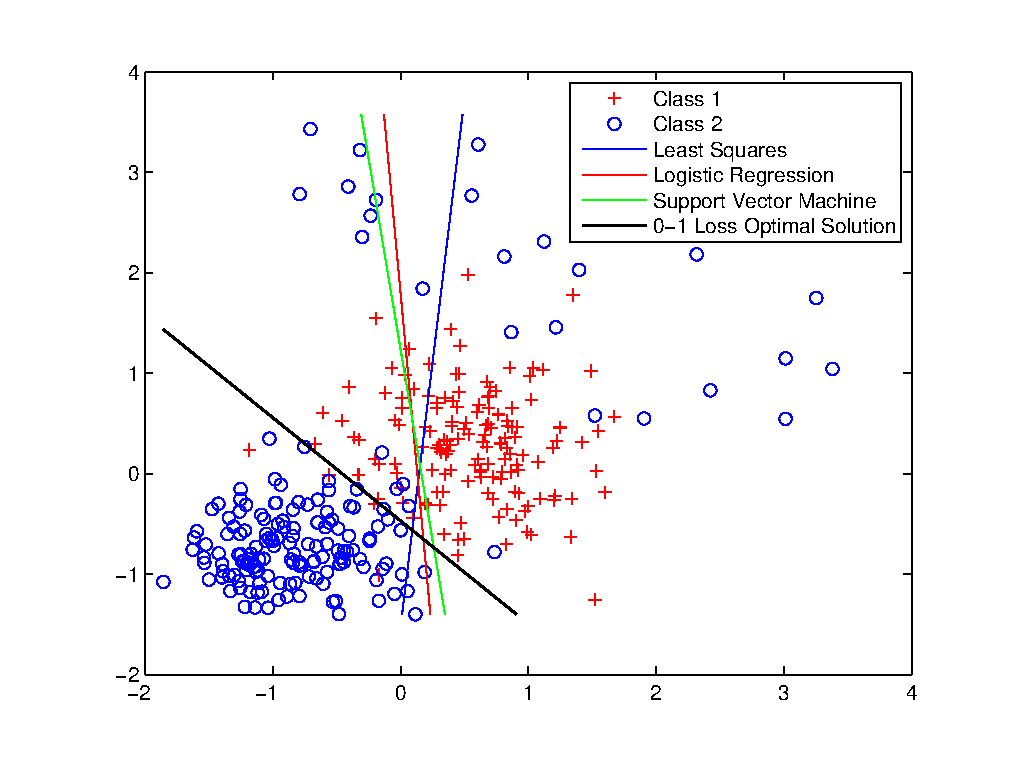
\includegraphics[width=0.50\textwidth]{images/fig11_svm_failure2.eps}
\caption{
Failure of common classifiers in the presence of outliers. 
The plot shows 300 training data points of two classes, 10\% of which are outliers. The least squares (blue line), logistic regression (red line) and support vector machine (green line) are all influenced by outliers and make around 61 classification errors, whereas the minimum of this number is 39 given by the black line corresponding to the optimal 0--1 loss solution.
}
\label{fig:svm_failure}
\end{figure}

It is known that most state-of-the-art classification methods including support vector machines suffer from the presence of outliers in the training set ~\cite{wu07}. This is illustrated in Figure \ref{fig:svm_failure}, where it can be seen that the line given by the least squares, support vector machine, and logistic regression methods clearly fail to separate the two classes at an optimal boundary. In some context, such failure could lead to a catastrophic amount of cost. Examples include testing whether a patient has cancer, or testing whether a locomotive wheel has crack. Outliers in these cases may come from abnormal noise or defect of equipments, from human mistakes, etc. These examples show that classifiers which are robust to outliers are needed. 

One approach to solve this problem is to use 0--1 loss, because this loss is robust to outliers. 0--1 loss basically counts the number of misclassifications regardless of the distance of any point to the decision boundary, hence outliers are treated in the same way as for any other points. This fact is illustrated in Figure \ref{fig:losses}. The minimum of 0--1 loss, therefore, coincides with the minimal number of classification errors. Thus, the decision boundary corresponding to the optimal 0--1 loss solution always gives the minimal misclassification rate for the training dataset. This is demonstrated by the black line in Figure \ref{fig:svm_failure}.

\begin{figure}[!ht]
\centering
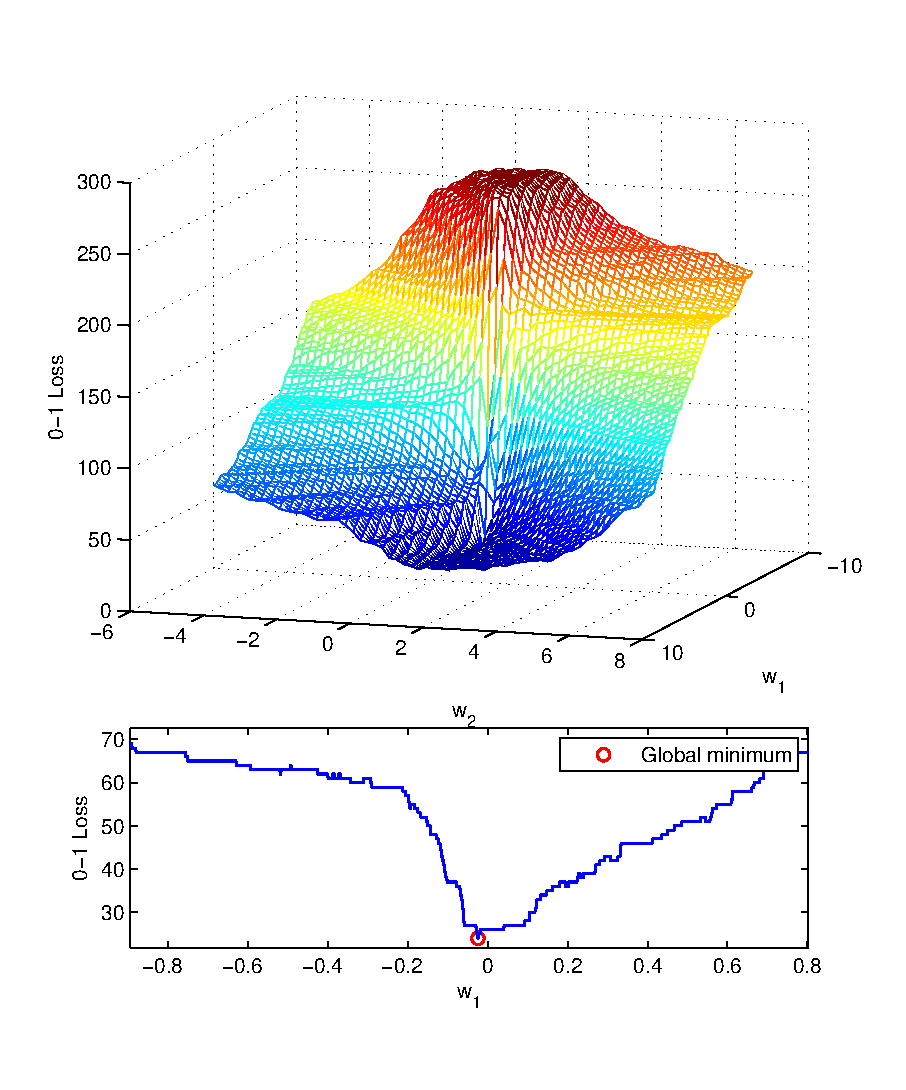
\includegraphics[width=0.50\textwidth]{images/fig14_complexshape.eps}
\caption{
The complex shape of 0--1 loss function. 
The top figure plots 0--1 loss function of a two-dimensional dataset as a function of two varying weights $w_1$ and $w_2$ (that control the decision boundary). The bottom figure plots the same function in more detailed scale with $w_2$ held fixed at optimal value. As can be seen, the 0--1 loss function has a complex shape with numerous local optima, which make the task of finding its global optimum hard. Practical datasets often have many more dimensions causing even more complicated shape.
}
\label{fig:complex_shape}
\end{figure}

\begin{figure}[here]
\centering
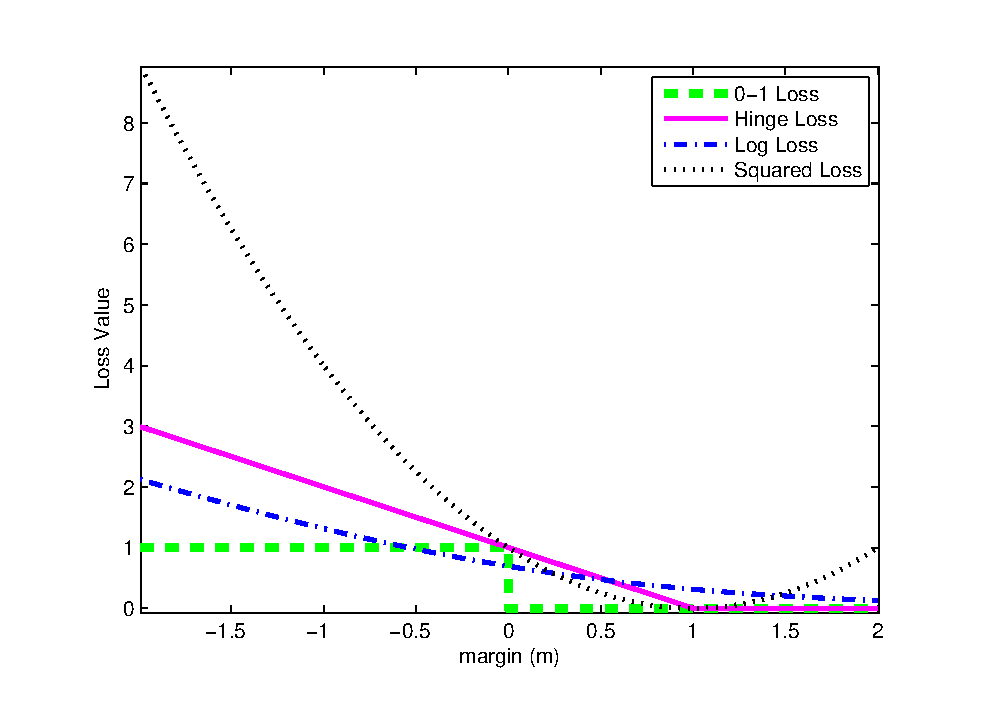
\includegraphics[width=0.50\textwidth]{images/fig13_losses.eps}
\caption{
0--1 loss versus some other losses. In this figure, the loss values are plotted as a function of margin $m$ representing some distance from a point to the decision boundary. A point is misclassified if and only if the corresponding margin is negative. Hinge loss is used by support vector machine, log loss by logistic regression, and squared loss by linear regression. It can be seen that for these losses, the more negative margin, the more loss value. In contrast, 0--1 loss is invariant to changes of the margin, as long as the margin sign stays the same.
}
\label{fig:losses}
\end{figure}

In spite of its importance, very little attempt has ever been made to construct methods for 0--1 loss optimization. This is due to the fact that the 0--1 loss is highly non-convex non-differentiable with many local optima, as shown in Figure \ref{fig:complex_shape}. In fact, it is NP--hard to optimize 0--1 loss directly \cite{Feldman,nphard}, and most of the current algorithms solve this problem by minimizing a convex surrogate of the 0--1 loss function, because convexity makes them computationally efficient \cite{Bartlett}. However, this leads to the problem with outliers as has been discussed previously. 

This thesis endeavors to explore some approaches to the problem of direct optimization of the 0--1 loss function for linear binary classification. We next discuss concrete objectives of the thesis.


%%===============================================
\subsection{Objectives}
\label{sec:intro.objectives}

Motivated by the importance of a method for finding or approximating the optimal solution of the 0--1 loss function for linear binary classification discussed in the previous section, this thesis aims to study in detail several approaches to solve this problem directly. More specifically, the objectives of this thesis are as follows:

\begin{enumerate}[ (i)]

\item {\bf To examine three different approaches to solve the problem:}  branch and bound, combinatorial search, and the smooth relaxation of 0--1 loss function.

\item {\bf To identify and analyze different heuristics} that help to prune the search space and/or increase the efficiency for the branch and bound and the combinatorial search approach. 

\item {\bf To find a method to optimize the function} resulting from the smooth relaxation of the 0--1 loss function. 

\item {\bf To design anytime algorithms} based on the above studies and analyze their complexity. 

\item {\bf To perform comprehensive testing} on both synthetic and real-world datasets to compare the proposed algorithms based on 0--1 loss with existing algorithms based on surrogate losses. 
 
\end{enumerate}



%%===============================================
\subsection{Major Contributions}
\label{sec:intro.contributions}

The followings are some of the major contributions of the thesis:

\begin{enumerate}[ (i)]

\item {\bf Development of several heuristics for the branch and bound search}, which enables the algorithm to solve problems of up to a few hundreds of data points (instead of tens) while guaranteeing the optimality of the returned solution. The first heuristic is the best-first strategy, which helps to find the optimal solution early by ordering the points for branching in decreasing distance to an approximated decision boundary. This heuristic essentially allows the algorithm to be anytime, increasing its practicality. The second heuristic is called loss propagation and helps to prune the search tree significantly using a convex hull created by points with assigned class in the current search path. This heuristic allows the algorithm to solve for optimal solution of problems of aforementioned size. 
 
\item {\bf Reformulation of the problem to enable combinatorial search}, which changes the search space from infinite and continuous to finite and discrete by considering only decision boundaries that go through all combinations, each of which contains a fixed number of points chosen from the dataset. A mechanism is developed to order these combinations such, that the best solution is likely to be found early, allowing an anytime algorithm, which can solve for the optimal solution of datasets of about a thousand points with low dimensionality. For bigger datasets or high dimensionality, an approximation algorithm is designed with two layers of approximation and polynomial worst-case running time, allowing it to solve problem of up to ten thousand data points. Practical tests on synthetic and real-world datasets show that these algorithms give good approximation to the optimal solution. 

\item {\bf Development of smooth loss}, which can approximate 0--1 loss to an arbitrarily level of precision. In contrast to 0--1 loss, the smooth loss function is continuous, differentiable, and its smoothness and approximation precision can be controlled by a constant. This essentially enabled the SLA algorithm, which optimizes the smooth loss function at increasing level of precision by repeatedly applying a modified version of the gradient descent method together with a range checker allowing the algorithm to escape from local optima. Tests on synthetic and real-world datasets show that SLA algorithm has similar approximation quality as that of the combinatorial search approximation, while its running time is significantly better: quadratic in worst-case but much faster on average. The SLA algorithm can solve problems of up to about a hundred thousand data points. 

\item {\bf Implementation of numerous tests} on both synthetic and real-world datasets to compare the performance of novel algorithms based on 0--1 loss with different existing algorithms based on surrogate losses. Tests showed that novel algorithms give significantly better 0--1 loss, and asserted the clear benefit of using classifiers based on 0--1 loss over the others in the presence of outliers. 

\end{enumerate}


%%===============================================
\subsection{Outline}
\label{sec:intro.outline}

The remaining chapters in this thesis are organized as follows:

\begin{itemize}

\item {\bf Chapter \ref{cha:background}} reviews linear binary classification and formulates the corresponding 0--1 loss optimization problem with a unified notation that will be used throughout the thesis. It then continues by reviewing existing methods to solve this problem. 

\item {\bf Chapter \ref{cha:branchandbound}} starts by providing the necessary foundation and tools for the construction of algorithms based on the branch and bound technique. It then examines different heuristics to improve the performance, most notably the best-first strategy, which help to find optimal solution early, and the loss propagation heuristic, which significantly reduces the search tree. A final algorithm with combined strengths of all analyzed heuristics is then presented together with its testing and performance analysis. The chapter is concluded by discussing the achievements and remaining challenges of this approach.  

\item {\bf Chapter \ref{cha:combinatorialsearch}} begins by describing and analyzing the idea that makes discretization of the search space of 0--1 loss optimization problem possible. It then proposes algorithms that use combinatorial search to find the optimal solution in the discretized search space, particularly an exhaustive anytime algorithm and an approximation algorithm. After that, detailed complexity analysis for each of the algorithms is provided, and the chapter is finalized with a summary.

\item {\bf Chapter \ref{cha:Smoothlossapprox}} focuses on developing and analyzing the smooth loss function that approximates the 0--1 loss function with a precision and smoothness controllable via a constant. After that, the SLA algorithm is developed to approximate 0--1 loss solution by repeatedly optimizing the smooth loss function at increasing level of precision. Then, the complexity of this algorithm is analyzed and tested, and the chapter is concluded by a summary.  

\item {\bf Chapter \ref{cha:results}} is devoted to testing on synthetic and real-world datasets and comparing the novel algorithms based on 0--1 loss with different existing algorithms based on surrogate losses. Firstly, the proposed algorithms are compared between themselves. Then, their representative, the SLA algorithm, is compared with existing algorithms such as logistic regression, support vector machine, Bayes point machine regarding the optimality of returned solution and the prediction accuracy. This chapter also analyzes anti-surrogate-loss datasets, for which algorithms based on surrogate losses performs badly, while  those based on 0--1 loss work well. A summary is given to finalize the chapter.

\item {\bf Chapter \ref{cha:conclusions}} summarizes all conclusions from this work and outlines directions for future research.

\end{itemize}

Altogether, this thesis represents an important step forward in direct optimization of 0--1 loss allowing the construction of linear binary classifiers that are robust to outliers.




%%% Local Variables: 
%%% mode: latex
%%% TeX-master: "thesis"
%%% End: 
